\chapter{Návrh vylepšení systému}
V této kapitole jsou navrženy způsoby vylepšení navrženého systému.


%%%%%%%%%%%%%%%%%%%%%%%%%%%%%%%%%%%%%%%%%%%%%%%%%%%%%%
\section{Návrh gatewaye verze 2}
Pro lepší mechanické uspořádání byla navržena verze 2 s navrženým plošným spojem (PCB).
Schéma zapojení je v obrázku \ref{fig:minigateway_schema} a plošný spoj je v obrázku \ref{fig:minigateway_plosnak}.
Je zde použit jiný vývojový kit NUCLEO-L432KC s výkonnějšim procesorem STM32L432KC, který má pinout stejný jako Arduino Nano, tedy je pod tímto názvem ve shcématu.
LoRa transceiver je použit RFM95w \cite{RFM95w} bez shieldu.
RS485 transceiver je použit LTC1480. 
Do zařízení je dále přidán externí stabilizátor, napěťový filtr, přepínač volitelné impedanční zakončení sítě RS485 a napěťové ochrany pro linky A, B a napájení. 

\begin{figure}[!h]
    \centering
    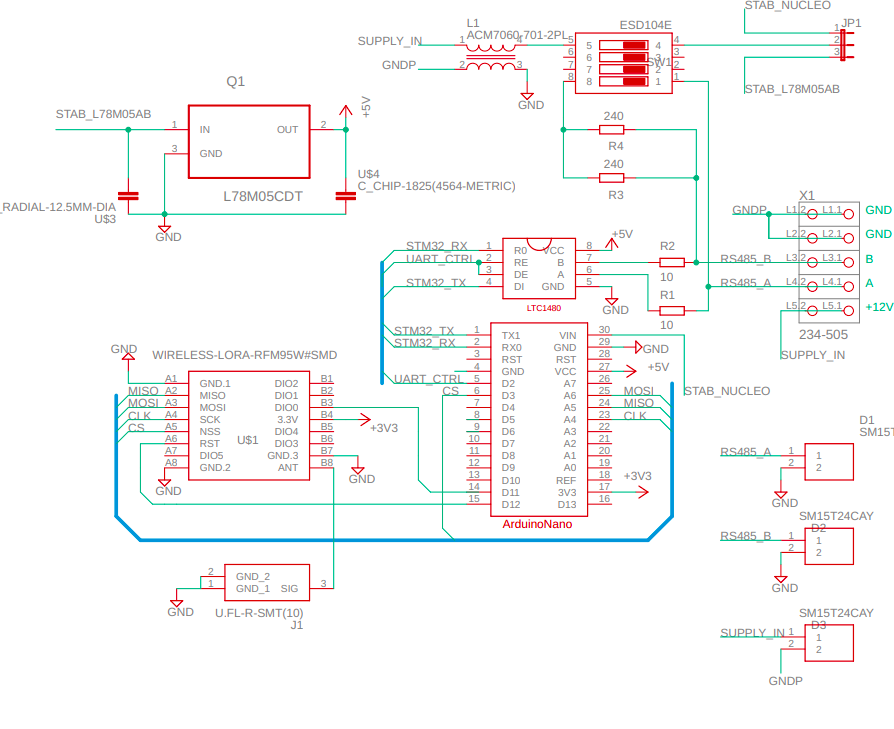
\includegraphics[width=1\textwidth]{minigateway_schema}
    \caption{Návrh gatewaye verze 2 - schéma}
    \label{fig:minigateway_schema}
\end{figure}

\begin{figure}[!h]
    \centering
    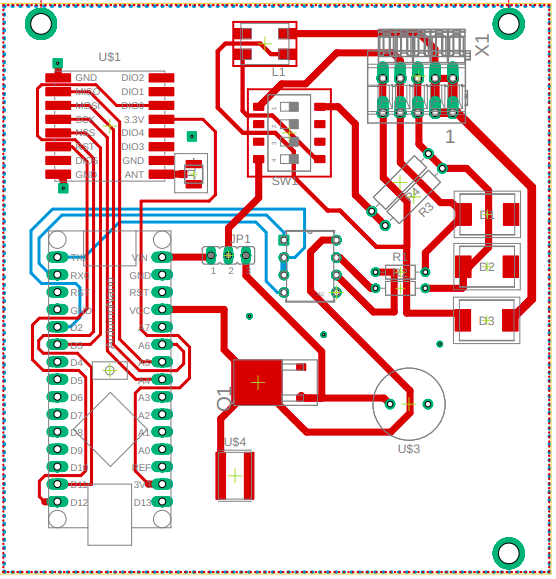
\includegraphics[width=0.7\textwidth]{minigateway_plosnak}
    \caption{Návrh gatewaye verze 2 - plošný spoj}
    \label{fig:minigateway_plosnak}
\end{figure}

Použitý procesor neobsahuje paměť EEPROM, tudíž pro ukládání konfigurace gatewaye a zařízení senzorové sítě je použita paměť flash.



